\documentclass[11pt]{article}
\usepackage{hw-solutions-common}
\usepackage{tikz}
\usetikzlibrary{arrows.meta,decorations.markings}

\begin{document}

\hwsolhead{Written HW 9}{Problem statements from Knight, \emph{Physics for Scientists and
Engineers} (5th ed., Global Edition), Chapter 30. $e=1.60\times10^{-19}$ C,
$m_p=1.67\times10^{-27}$ kg throughout.}

%============================================================
\problem{30.2}{3}{A 10-cm-long wire is pulled along a U-shaped conducting
rail in a perpendicular magnetic field. The total resistance of the wire and
rail is 0.20 $\Omega$. Pulling the wire at a steady speed of 4.0 m/s causes
4.0 W of power to be dissipated in the circuit. (a) How big is the pulling
force? (b) What is the strength of the magnetic field?}

\model{At a \emph{steady} speed the wire's net force is zero, so the pulling
force exactly balances the magnetic drag force. That means every joule of
work the puller does shows up as dissipated electrical power: $P=F_{\text{pull}}v$.
That alone gives part (a). For part (b), the motional emf is
$\varepsilon=B\ell v$, which drives a current $I=\varepsilon/R$ and dissipates
$P=\varepsilon^2/R=(B\ell v)^2/R$ --- solve that for $B$.}

\visualize{
\begin{center}
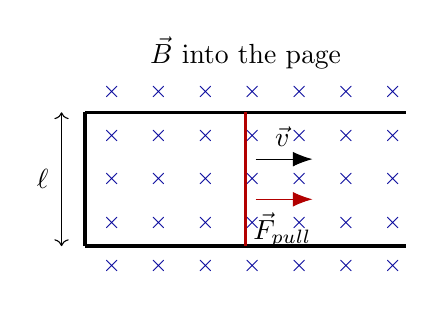
\begin{tikzpicture}[scale=0.85]
\foreach \x in {-2.0,-1.3,-0.6,0.1,0.8,1.5,2.2}{
  \foreach \y in {-1.3,-0.65,0,0.65,1.3}{
    \node[blue!60!black] at (\x,\y) {\footnotesize $\times$};
  }
}
\draw[very thick] (-2.4,1.0) -- (2.4,1.0);
\draw[very thick] (-2.4,-1.0) -- (2.4,-1.0);
\draw[very thick] (-2.4,-1.0) -- (-2.4,1.0);
\draw[very thick, red!70!black] (0,-1.0) -- (0,1.0);
\draw[<->] (-2.75,-1.0) -- (-2.75,1.0);
\node[left] at (-2.8,0) {$\ell$};
\draw[-{Latex[length=2.5mm]}] (0.15,0.3) -- (1.0,0.3);
\node[above] at (0.55,0.35) {$\vec v$};
\draw[-{Latex[length=2.5mm]}, red!70!black] (0.15,-0.3) -- (1.0,-0.3);
\node[below] at (0.55,-0.35) {$\vec F_{\text{pull}}$};
\node[above] at (0,1.5) {$\vec B$ into the page};
\end{tikzpicture}
\end{center}
The U-shaped rail and sliding wire form a closed loop; the wire of length
$\ell=10$ cm is dragged to the right at constant $v$, so the induced current
$I$ through resistance $R$ dissipates power $P$ exactly as fast as the
pulling force supplies it.}

\solve{(a)
\[
P=F_{\text{pull}}v \;\Rightarrow\; F_{\text{pull}}=\frac{P}{v}=
\frac{4.0\text{ W}}{4.0\text{ m/s}}=\boxed{1.0\text{ N}}.
\]
(b)
\[
P=\frac{(B\ell v)^2}{R} \;\Rightarrow\;
B=\frac{\sqrt{PR}}{\ell v}=\frac{\sqrt{(4.0\text{ W})(0.20\ \Omega)}}
{(0.10\text{ m})(4.0\text{ m/s})}=\frac{0.894}{0.40}=\boxed{2.2\text{ T}}.
\]}

\review{Check the two parts against each other: with $B=2.2$ T, the current
is $I=\varepsilon/R=B\ell v/R=(2.2)(0.10)(4.0)/0.20=4.5$ A, and
$F_{\text{pull}}=BI\ell=(2.2)(4.5)(0.10)=1.0$ N --- exactly the part (a)
answer, as it must be, since both routes describe the same steady-state
force balance. 2.2 T is a strong field (comparable to an MRI magnet), which
makes sense: dissipating 4.0 W through a fairly brisk 4.0 m/s pull with only
0.10 m of wire needs a hefty field to generate much current.}

%============================================================
\problem{30.11}{2}{The metal equilateral triangle in \textbf{Figure
EX30.11}, 20 cm on each side, is halfway into a 0.10 T magnetic field.
(a) What is the magnitude of the magnetic flux through the triangle? (b) If
the magnetic field strength decreases, what is the direction of the induced
current in the triangle?}

\model{Flux only accumulates where the field actually penetrates the loop:
here the field exists only in the \emph{left} half of the triangle (split by
its own vertical symmetry axis) --- the right half sits in a field-free
region and contributes nothing. So the relevant area for $\Phi=BA$ is just
that left half-triangle, a $30$--$60$--$90$ right triangle with base
$10$ cm (half of the $20$ cm side) and height equal to the full altitude of
the equilateral triangle, $20\sin60^\circ$ cm.}

\visualize{
\begin{center}
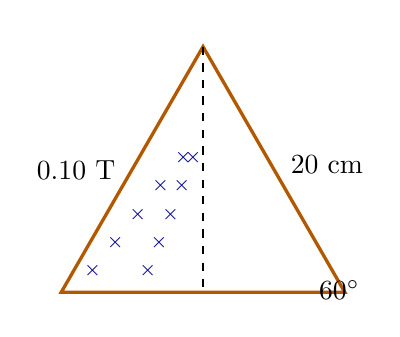
\begin{tikzpicture}[scale=1.8]
\coordinate (A) at (0,1.732);
\coordinate (B) at (-1,0);
\coordinate (C) at (1,0);
\foreach \y/\xs in {0.15/0.78,0.35/0.62,0.55/0.46,0.75/0.30,0.95/0.14}{
  \node[blue!60!black] at (-\xs,\y) {\scriptsize$\times$};
  \pgfmathsetmacro{\xmid}{\xs/2}
  \node[blue!60!black] at (-\xmid,\y) {\scriptsize$\times$};
}
\draw[very thick, orange!70!black] (A) -- (B) -- (C) -- cycle;
\draw[dashed] (A) -- (0,0);
\node[above] at (A) {};
\node[below left] at (-0.55,1.0) {$0.10$ T};
\node[below right] at (0.75,0.15) {$60^\circ$};
\node[right] at (0.55,0.9) {$20$ cm};
\end{tikzpicture}
\end{center}
The dashed line is the triangle's vertical symmetry axis; only the half
marked with $\times$'s (left of the dashed line) lies in the field --- the
right half is field-free. That half-triangle has base $0.10$ m and height
$(0.20\text{ m})\sin60^\circ=0.1732$ m.}

\solve{(a)
\[
A_{\text{half}}=\tfrac12(\text{base})(\text{height})=\tfrac12(0.10\text{
m})(0.1732\text{ m})=8.66\times10^{-3}\ \text{m}^2
\]
\[
\Phi=BA_{\text{half}}=(0.10\text{ T})(8.66\times10^{-3}\
\text{m}^2)=\boxed{8.7\times10^{-4}\ \text{Wb}}.
\]
(b) The flux into the loop is decreasing. By Lenz's law the induced current
opposes that decrease, so its own field must point \emph{into} the loop (the
same direction as the original field) to try to prop the flux back up. By
the right-hand rule, that requires the induced current to flow
\boxed{\text{clockwise}}.}

\review{Sanity check on the area: the full equilateral triangle has area
$\frac{\sqrt3}{4}(0.20\text{ m})^2=1.73\times10^{-2}\ \text{m}^2$, and half of
that is $8.66\times10^{-3}\ \text{m}^2$ --- matches. The more important point
is conceptual: even though the whole triangle is one conducting loop, only
the half that's actually immersed in $\vec B$ contributes to $\Phi$ ---
$\Phi=\int\vec B\cdot d\vec A$ is zero wherever $\vec B$ is zero, loop or no
loop.}

%============================================================
\problem{30.12}{3}{The current in the solenoid of \textbf{Figure EX30.12} is
increasing. The solenoid is surrounded by a conducting loop. Is there a
current in the loop? If so, is the loop current cw or ccw?}

\model{A long solenoid's field is (nearly) confined to its interior, so a
loop encircling the solenoid --- even though its own area is a bit larger
than the solenoid's cross section --- still captures essentially the full
internal flux, since almost no field lines exist outside to \emph{not} be
captured. As $I_{\text{sol}}$ grows, that enclosed flux grows, and Lenz's law
says the loop's induced current opposes the increase.}

\visualize{
\begin{center}
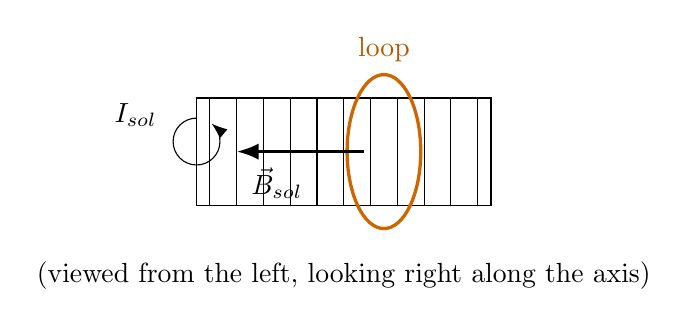
\begin{tikzpicture}[scale=0.85]
\draw (-2.2,-0.8) rectangle (2.2,0.8);
\foreach \x in {-2.0,-1.6,-1.2,-0.8,-0.4,0,0.4,0.8,1.2,1.6,2.0}{
  \draw (\x,-0.8) -- (\x,0.8);
}
\draw[very thick, orange!80!black] (0.6,0) ellipse (0.55 and 1.15);
\node[orange!70!black, above] at (0.6,1.2) {loop};
\draw[-{Latex[length=2.8mm]}, very thick] (0.3,0) -- (-1.6,0);
\node[below] at (-1.0,-0.1) {$\vec B_{\text{sol}}$};
\draw[-{Latex[length=2mm]}] (-2.2,0.5) arc (90:410:0.35);
\node[left] at (-2.65,0.55) {$I_{\text{sol}}$};
\node[below] at (0,-1.5) {(viewed from the left, looking right along the axis)};
\end{tikzpicture}
\end{center}
As shown, $I_{\text{sol}}$ circulates counterclockwise when viewed from the
left end looking right along the axis, which by the right-hand rule drives
$\vec B_{\text{sol}}$ pointing \emph{left} (toward that same viewer) inside
the solenoid.}

\solve{Since $I_{\text{sol}}$ is increasing, $\vec B_{\text{sol}}$ (pointing
left) is growing stronger, so the leftward flux through the surrounding loop
is increasing. By Lenz's law the loop's induced current must create a field
that opposes that increase --- i.e., a field pointing \emph{right} inside the
loop. Applying the right-hand rule to a rightward-pointing field (same
left-looking-right viewpoint) requires the current to circulate
\boxed{\text{clockwise}}.}

\review{Yes, there is an induced current, and its direction is opposite the
sense of $I_{\text{sol}}$ itself (ccw in the solenoid, cw in the loop) ---
makes sense, since the loop is actively fighting against the solenoid's
growing field. Notice the loop's exact radius never entered the reasoning:
as long as it's larger than the solenoid and coaxial with it, it encloses
the same flux a snug-fitting loop would, since the field just outside a long
solenoid is essentially zero.}

%============================================================
\problem{30.16}{3}{A 1000-turn coil of wire 1.0 cm in diameter is in a
magnetic field that increases from 0.10 T to 0.30 T in 10 ms. The axis of
the coil is parallel to the field. What is the emf of the coil?}

\model{With the coil's axis parallel to $\vec B$, the flux through each turn
is simply $\Phi=BA$ (no $\cos\theta$ factor needed). Faraday's law for an
$N$-turn coil gives $\varepsilon=N\left|\dfrac{d\Phi}{dt}\right|=NA\left|\dfrac{\Delta
B}{\Delta t}\right|$, since only $B$ --- not the coil's area or orientation
--- is changing.}

\visualize{
\begin{center}
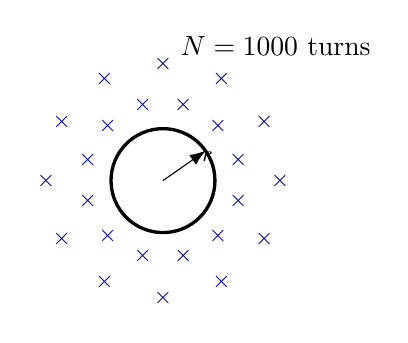
\begin{tikzpicture}[scale=1.1]
\foreach \ang in {0,30,...,330}{
  \node[blue!60!black] at (\ang:1.35) {\footnotesize$\times$};
}
\foreach \ang in {15,45,...,345}{
  \node[blue!60!black] at (\ang:0.9) {\footnotesize$\times$};
}
\draw[very thick] (0,0) circle (0.6);
\draw[-{Latex[length=2mm]}] (0,0) -- (35:0.6);
\node[above right] at (17:0.35) {\footnotesize $r$};
\node at (1.3,1.55) {$N=1000$ turns};
\end{tikzpicture}
\end{center}
The coil's diameter is $1.0$ cm, so $r=0.50$ cm $=0.0050$ m.}

\solve{
\[
A=\pi r^2=\pi(0.0050\text{ m})^2=7.85\times10^{-5}\ \text{m}^2
\]
\[
\left|\frac{\Delta B}{\Delta t}\right|=\frac{0.30\text{ T}-0.10\text{
T}}{10\times10^{-3}\text{ s}}=20\ \text{T/s}
\]
\[
\varepsilon=NA\left|\frac{\Delta B}{\Delta t}\right|=(1000)(7.85\times10^{-5}\
\text{m}^2)(20\ \text{T/s})=\boxed{1.6\ \text{V}}.
\]}

\review{A single turn in the same tiny (1.0-cm-diameter) coil would only
produce $1.6\ \text{mV}$ --- it's entirely the $N=1000$ multiplier that
turns a modest field ramp into a usable 1.6 V. Also notice the sign of
$\Delta B$ never entered the calculation; Faraday's law only cares about the
\emph{magnitude} of the rate of change for the emf's size (its direction is
a separate, Lenz's-law question).}

%============================================================
\problem{30.17}{4}{\textbf{CALC} A 5.0-cm-diameter coil has 20 turns and a
resistance of 0.50 $\Omega$. A magnetic field perpendicular to the coil is
$B=0.020t+0.010t^2$, where $B$ is in tesla and $t$ is in seconds. (a) Find
an expression for the induced current $I(t)$ as a function of time. (b)
Evaluate $I$ at $t=5$ s and $t=10$ s.}

\model{The field is perpendicular to the coil (so $\Phi=BA$ again) but now
changes with time according to a given function, so
$\varepsilon(t)=NA\left|\dfrac{dB}{dt}\right|$ must be found by
differentiating $B(t)$ first. Ohm's law then converts that emf into a
current, $I(t)=\varepsilon(t)/R$.}

\visualize{
\begin{center}
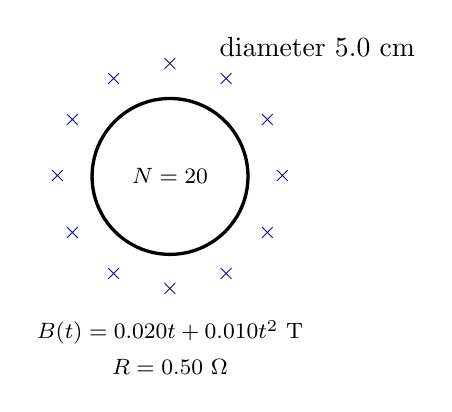
\begin{tikzpicture}[scale=1.1]
\foreach \ang in {0,30,...,330}{
  \node[blue!60!black] at (\ang:1.3) {\footnotesize$\times$};
}
\draw[very thick] (0,0) circle (0.9);
\node at (0,0) {\footnotesize $N=20$};
\node[below] at (0,-1.55) {\footnotesize $B(t)=0.020t+0.010t^2$ T};
\node[below] at (0,-2.0) {\footnotesize $R=0.50\ \Omega$};
\node at (1.7,1.5) {diameter $5.0$ cm};
\end{tikzpicture}
\end{center}
The coil's radius is $2.5$ cm $=0.025$ m, so $A=\pi(0.025\text{
m})^2=1.96\times10^{-3}\ \text{m}^2$.}

\solve{(a)
\[
\frac{dB}{dt}=0.020+0.020t\ \ \text{(T/s)}
\]
\[
\varepsilon(t)=NA\left|\frac{dB}{dt}\right|=(20)(1.96\times10^{-3}\
\text{m}^2)(0.020+0.020t) = 7.85\times10^{-4}(1+t)\ \text{V}
\]
\[
I(t)=\frac{\varepsilon(t)}{R}=\frac{7.85\times10^{-4}(1+t)\
\text{V}}{0.50\ \Omega} = \boxed{1.6\times10^{-3}(1+t)\ \text{A}}.
\]
(b)
\[
I(5\text{ s}) = (1.57\times10^{-3})(1+5) = \boxed{9.4\times10^{-3}\
\text{A}}
\]
\[
I(10\text{ s}) = (1.57\times10^{-3})(1+10) = \boxed{1.7\times10^{-2}\
\text{A}}.
\]}

\review{$I(t)$ comes out perfectly linear in $t$, which makes sense: $dB/dt$
itself is linear in $t$ (since $B(t)$ has a $t^2$ term), and everything else
in $\varepsilon(t)=NA|dB/dt|$ is a constant. Check the ratio:
$I(10)/I(5)=11/6=1.83$, and indeed $(1+10)/(1+5)=11/6$ --- consistent. Even
though the field $B(t)$ itself is always increasing, it's really the
\emph{rate of change} $dB/dt$ that sets the current, and that rate keeps
climbing too (the field's growth is accelerating), which is why $I$ keeps
climbing at $t=10$ s rather than leveling off.}

%============================================================
\problem{30.18}{3}{\textbf{INT} The magnetic field in \textbf{Figure
EX30.18} is decreasing at the rate $0.10$ T/s. What is the acceleration
(magnitude and direction) of a proton initially at rest at points 1 to 4?}

\model{A changing $B$ induces a circulating electric field even with no wire
present (Section 30.6). Inside a circular field region of radius $R$, that
induced field has magnitude $E(r)=\dfrac{r}{2}\left|\dfrac{dB}{dt}\right|$ at
radial distance $r$ from the center, directed tangentially; the sense
(cw/ccw) comes from Lenz's law, as if a loop \emph{were} there. A proton at
rest then simply obeys Newton's second law with this electric force:
$\vec a=e\vec E/m_p$, in the same direction as $\vec E$ (positive charge).}

\visualize{
\begin{center}
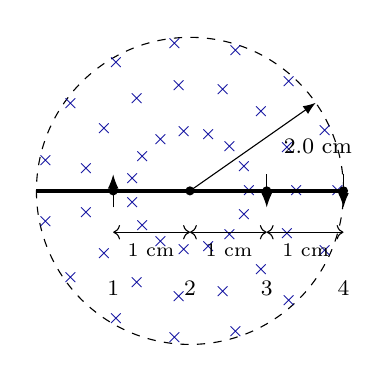
\begin{tikzpicture}[scale=1.5]
\draw[dashed] (0,0) circle (1.3);
\foreach \ang in {0,24,...,336}{
  \foreach \rad in {0.5,0.9,1.25}{
    \node[blue!60!black] at (\ang:\rad) {\scriptsize$\times$};
  }
}
\draw[very thick] (-1.3,0) -- (1.3,0);
\foreach \x in {-0.65,0,0.65,1.3}{
  \fill (\x,0) circle (1.1pt);
}
\draw[-{Latex[length=1.6mm]}] (0,0) -- (35:1.3);
\node[above right] at (18:0.75) {\footnotesize $2.0$ cm};
\draw[-{Latex[length=1.8mm]}] (-0.65,-0.14) -- (-0.65,0.14);
\draw[-{Latex[length=1.8mm]}] (0.65,0.14) -- (0.65,-0.14);
\draw[-{Latex[length=1.8mm]}] (1.3,0.14) -- (1.3,-0.14);
\draw[<->] (-0.65,-0.35) -- (0,-0.35); \node[below] at (-0.33,-0.37) {\scriptsize$1$ cm};
\draw[<->] (0,-0.35) -- (0.65,-0.35); \node[below] at (0.33,-0.37) {\scriptsize$1$ cm};
\draw[<->] (0.65,-0.35) -- (1.3,-0.35); \node[below] at (0.98,-0.37) {\scriptsize$1$ cm};
\foreach \x/\lab in {-0.65/1,0/2,0.65/3,1.3/4}{
  \node[below] at (\x,-0.68) {\footnotesize \lab};
}
\end{tikzpicture}
\end{center}
$\vec B$ points into the page and is decreasing, so by Lenz's law the
induced $\vec E$ circulates \emph{clockwise} (to drive a current that would
try to maintain the inward flux). Points 1--4 lie 1 cm apart on a line
through the center (point 2); clockwise circulation points \emph{up} on the
left side (points 1) and \emph{down} on the right side (points 3, 4), as
drawn.}

\solve{
\[
a(r)=\frac{eE(r)}{m_p}=\frac{er}{2m_p}\left|\frac{dB}{dt}\right|
\]
Point 1 ($r=1.0$ cm $=0.010$ m, up):
\[
a_1=\frac{(1.60\times10^{-19}\text{ C})(0.010\text{
m})(0.10\text{ T/s})}{2(1.67\times10^{-27}\text{ kg})} =
\boxed{4.8\times10^4\ \text{m/s}^2\text{, up}}.
\]
Point 2 ($r=0$, the center):
\[
\boxed{a_2=0}.
\]
Point 3 ($r=1.0$ cm, down): same magnitude as point 1, opposite side,
\[
a_3=\boxed{4.8\times10^4\ \text{m/s}^2\text{, down}}.
\]
Point 4 ($r=2.0$ cm $=0.020$ m, down): twice the radius of point 3,
\[
a_4=\boxed{9.6\times10^4\ \text{m/s}^2\text{, down}}.
\]}

\review{$a(r)$ is exactly linear in $r$ --- doubling the radius (point 3 to
point 4) exactly doubles the acceleration. This is the same ``uniform
source spread over a disk'' scaling that shows up for $\vec E$ inside a
uniformly charged sphere or $\vec B$ inside a uniform current-carrying wire:
the induced field grows linearly out from the center, then (outside the
field region, not asked here) would fall off as $1/r$ instead. Point 2 sits
exactly on the axis of symmetry, where the tangential contributions from all
sides cancel --- a proton dropped there, unlike anywhere else inside the
field region, would feel nothing at all.}

\end{document}
